\documentclass[a4paper, 10pt]{article}
\usepackage[utf8]{inputenc}
\usepackage[spanish]{babel}
\usepackage{graphicx}
\usepackage{geometry}
\usepackage{listings}
\usepackage{amsmath}
\usepackage{amsfonts}
\usepackage{amssymb}
\usepackage{caratula}

\newcommand{\Z}{\mathbb{Z}}
\def\code#1{\texttt{#1}}
\newcommand\tab[1][0.5cm]{\hspace*{#1}}

\geometry{a4paper, margin=0.7in}

\begin{document}
    %Caratula
    \pagenumbering{gobble}
    \newpage

    \begin{center}
        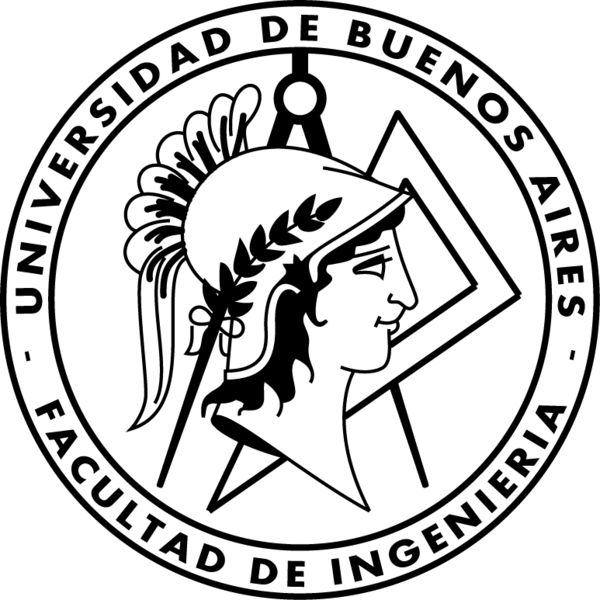
\includegraphics{images/logo}
    \end{center}

    \materia{Teoría de Algoritmos 2}
    \submateria{Segundo Cuatrimestre 2017}
    \titulo{Trabajo Práctico 1}

    \integrante{Rodrigo De Rosa}{97799}{rodrigoderosa@outlook.com}
    \integrante{Marcos Schapira}{97934}{schapiramarcos@gmail.com}
    \integrante{Facundo Guerrero}{97981}{facundoiguerrero@gmail.com}
    \maketitle
    %Fin caratula
    %Table of contents
    \newpage
    \pagenumbering{roman}
    \tableofcontents
    %Fin table of contents
    %Informe
    \newpage
	\pagenumbering{arabic}
	
	\section{Rabin - Karp}
		
		\emph{Algoritmo Michael O. Rabin and Richard M. Karp 1987}
		
		\subsection{Funcionamiento}
		\tab La idea del algoritmo es muy simple. Basándose en la estructura del algoritmo naïve, este 				agrega un paso previo que compara los strings por valores de hash. Para esto precisa una función de 		hash que se busca que compare entre valores lo mas rápido posible. Esto tiene el potencial 					beneficio de acortar los tiempos de comparación entre strings mientras que agrega la complejidad 			del calculo previo del valor de hash para cada string.
		
		\subsection{Implementación}
		
		La implementación es muy simple. Primero calcula el valor de hash para el patrón a buscar. Luego recorre el texto calculando el valor de hash para la palabra a buscar. Compara ambos valores y si dan iguales entonces compara si las palabras son realmente iguales o no. Para ganar mayor velocidad se utilizo la librería pyhash \footnote{https://github.com/flier/pyfasthash} que contiene implementaciones en C/C++ para mejor eficiencia de algoritmos no criptográficos. De estos se usaron (todos de 32 bits): FNV, Murmur Hash, City Hash, Spooky Hash.
		
		\subsection{Complejidad}
		
		En el peor de los casos, el algoritmo compara cada string del texto contra el patrón teniendo un orden de $O(nm)$ donde n es la longitud del texto y p la del patron. Esto ocurre en el caso en donde se use una función de hash muy mala. Con una función de hash relativamente buena se mejora el orden a $O(n+m)$.
		
		\subsection{Investigación y aplicaciones}
		
		Este algoritmo no es utilizado para Simple Matching ya que resulta poco eficiente. Esto se debe que  el costo que tiene para calcular las claves entre algoritmos resulta mayor en relación al beneficio que se obtiene de la rapidez para comparar strings. Investigando sobre sus aplicaciones en el ámbito profesional se encuentra que este algoritmo resulta particularmente útil para el problema de múltiple string matching, mas es así en la búsqueda de plagios. Esto es, teniendo un texto A y un texto B, comparar que tan semejante resulta A contra B.
		
		\subsection{Conclusiones}
		
		Para simple matching este algoritmo resulta increíblemente ineficiente dando los peores tiempos ejecución. Sin embargo para múltiple matching es un muy buen algoritmo. Como optimización se siguiere sacar la parte en donde se verifica que la los valores de hashes que tuvieron match sean realmente iguales. Esto funcionaria sin problemas con una función de hashing perfecto (pero al entiza la ejecución), sin embargo si no lo es el algoritmo pasaría a ser randomizado ya que las funciones de hash utilizadas en este caso garantizan pocas colisiones pero no es imposible que ocurran.    	
		
\end{document}
